\documentclass[11pt]{article}
\usepackage{amssymb,amsmath}
\usepackage{color,soul}
\usepackage{tikz,ifthen,calc}
\usetikzlibrary{positioning}
\usetikzlibrary{shapes}
\usetikzlibrary{shapes.symbols,patterns}
\usetikzlibrary{calc,through,backgrounds}
\usetikzlibrary{decorations.pathreplacing}
\usetikzlibrary{shapes.geometric, arrows}

\begin{document}

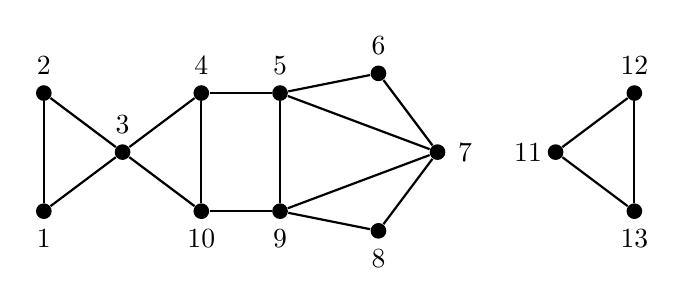
\begin{tikzpicture}[scale=0.5]
%
\begin{scope}[
every node/.style={fill=black,circle,inner sep=2pt},
every edge/.style={draw=black,thick}]
%
\node(v1) at (0,0) {};
\node(v2) at (0,3) {};
\node(v3) at (2,1.5) {};
\node(v4) at (4,3) {};
\node(v5) at (6,3) {};
\node(v6) at (8.5,3.5) {};
\node(v7) at (10,1.5) {};
\node(v8) at (8.5,-0.5) {};
\node(v9) at (6,0) {};
\node(v10) at (4,0) {};
\node(v11) at (13,1.5) {};
\node(v12) at (15,3) {};
\node(v13) at (15,0) {};

\path (v1) [-] edge (v2);
\path (v1) [-] edge (v3);
\path (v2) [-] edge (v3);
\path (v3) [-] edge (v4);
\path (v3) [-] edge (v10);
\path (v4) [-] edge (v10);
\path (v4) [-] edge (v5);
\path (v5) [-] edge (v9);
\path (v5) [-] edge (v6);
\path (v5) [-] edge (v7);
\path (v6) [-] edge (v7);
\path (v7) [-] edge (v8);
\path (v7) [-] edge (v9);
\path (v8) [-] edge (v9);
\path (v9) [-] edge (v10);
\path (v11) [-] edge (v12);
\path (v11) [-] edge (v13);
\path (v12) [-] edge (v13);
\end{scope}

\node () at (0,-0.7) {$1$};
\node () at (0,3.7) {$2$};
\node () at (2,2.2) {$3$};
\node () at (4,3.7) {$4$};
\node () at (6,3.7) {$5$};
\node () at (8.5,4.2) {$6$};
\node () at (10.7,1.5) {$7$};
\node () at (8.5,-1.2) {$8$};
\node () at (6,-0.7) {$9$};
\node () at (4,-0.7) {$10$};
\node () at (12.3,1.5) {$11$};
\node () at (15,3.7) {$12$};
\node () at (15,-0.7) {$13$};
%
\end{tikzpicture}

\end{document}